\documentclass[twoside]{book}

% Packages required by doxygen
\usepackage{fixltx2e}
\usepackage{calc}
\usepackage{doxygen}
\usepackage[export]{adjustbox} % also loads graphicx
\usepackage{graphicx}
\usepackage[utf8]{inputenc}
\usepackage{makeidx}
\usepackage{multicol}
\usepackage{multirow}
\PassOptionsToPackage{warn}{textcomp}
\usepackage{textcomp}
\usepackage[nointegrals]{wasysym}
\usepackage[table]{xcolor}

% Font selection
\usepackage[T1]{fontenc}
\usepackage[scaled=.90]{helvet}
\usepackage{courier}
\usepackage{amssymb}
\usepackage{sectsty}
\renewcommand{\familydefault}{\sfdefault}
\allsectionsfont{%
  \fontseries{bc}\selectfont%
  \color{darkgray}%
}
\renewcommand{\DoxyLabelFont}{%
  \fontseries{bc}\selectfont%
  \color{darkgray}%
}
\newcommand{\+}{\discretionary{\mbox{\scriptsize$\hookleftarrow$}}{}{}}

% Page & text layout
\usepackage{geometry}
\geometry{%
  a4paper,%
  top=2.5cm,%
  bottom=2.5cm,%
  left=2.5cm,%
  right=2.5cm%
}
\tolerance=750
\hfuzz=15pt
\hbadness=750
\setlength{\emergencystretch}{15pt}
\setlength{\parindent}{0cm}
\setlength{\parskip}{3ex plus 2ex minus 2ex}
\makeatletter
\renewcommand{\paragraph}{%
  \@startsection{paragraph}{4}{0ex}{-1.0ex}{1.0ex}{%
    \normalfont\normalsize\bfseries\SS@parafont%
  }%
}
\renewcommand{\subparagraph}{%
  \@startsection{subparagraph}{5}{0ex}{-1.0ex}{1.0ex}{%
    \normalfont\normalsize\bfseries\SS@subparafont%
  }%
}
\makeatother

% Headers & footers
\usepackage{fancyhdr}
\pagestyle{fancyplain}
\fancyhead[LE]{\fancyplain{}{\bfseries\thepage}}
\fancyhead[CE]{\fancyplain{}{}}
\fancyhead[RE]{\fancyplain{}{\bfseries\leftmark}}
\fancyhead[LO]{\fancyplain{}{\bfseries\rightmark}}
\fancyhead[CO]{\fancyplain{}{}}
\fancyhead[RO]{\fancyplain{}{\bfseries\thepage}}
\fancyfoot[LE]{\fancyplain{}{}}
\fancyfoot[CE]{\fancyplain{}{}}
\fancyfoot[RE]{\fancyplain{}{\bfseries\scriptsize Generated by Doxygen }}
\fancyfoot[LO]{\fancyplain{}{\bfseries\scriptsize Generated by Doxygen }}
\fancyfoot[CO]{\fancyplain{}{}}
\fancyfoot[RO]{\fancyplain{}{}}
\renewcommand{\footrulewidth}{0.4pt}
\renewcommand{\chaptermark}[1]{%
  \markboth{#1}{}%
}
\renewcommand{\sectionmark}[1]{%
  \markright{\thesection\ #1}%
}

% Indices & bibliography
\usepackage{natbib}
\usepackage[titles]{tocloft}
\setcounter{tocdepth}{3}
\setcounter{secnumdepth}{5}
\makeindex

% Hyperlinks (required, but should be loaded last)
\usepackage{ifpdf}
\ifpdf
  \usepackage[pdftex,pagebackref=true]{hyperref}
\else
  \usepackage[ps2pdf,pagebackref=true]{hyperref}
\fi
\hypersetup{%
  colorlinks=true,%
  linkcolor=blue,%
  citecolor=blue,%
  unicode%
}

% Custom commands
\newcommand{\clearemptydoublepage}{%
  \newpage{\pagestyle{empty}\cleardoublepage}%
}

\usepackage{caption}
\captionsetup{labelsep=space,justification=centering,font={bf},singlelinecheck=off,skip=4pt,position=top}

%===== C O N T E N T S =====

\begin{document}

% Titlepage & ToC
\hypersetup{pageanchor=false,
             bookmarksnumbered=true,
             pdfencoding=unicode
            }
\pagenumbering{alph}
\begin{titlepage}
\vspace*{7cm}
\begin{center}%
{\Large Editor G\+UI Table \\[1ex]\large 1.\+0 }\\
\vspace*{1cm}
{\large Generated by Doxygen 1.8.14}\\
\end{center}
\end{titlepage}
\clearemptydoublepage
\pagenumbering{roman}
\tableofcontents
\clearemptydoublepage
\pagenumbering{arabic}
\hypersetup{pageanchor=true}

%--- Begin generated contents ---
\chapter{Namespace Index}
\section{Namespace List}
Here is a list of all documented namespaces with brief descriptions\+:\begin{DoxyCompactList}
\item\contentsline{section}{\mbox{\hyperlink{namespace_editor_g_u_i_table}{Editor\+G\+U\+I\+Table}} }{\pageref{namespace_editor_g_u_i_table}}{}
\end{DoxyCompactList}

\chapter{Hierarchical Index}
\section{Class Hierarchy}
This inheritance list is sorted roughly, but not completely, alphabetically\+:\begin{DoxyCompactList}
\item \contentsline{section}{G\+U\+I\+Extensions.\+G\+U\+I\+Table\+State}{\pageref{class_g_u_i_extensions_1_1_g_u_i_table_state}}{}
\item I\+Comparable\begin{DoxyCompactList}
\item \contentsline{section}{G\+U\+I\+Extensions.\+Table\+Entry}{\pageref{class_g_u_i_extensions_1_1_table_entry}}{}
\begin{DoxyCompactList}
\item \contentsline{section}{G\+U\+I\+Extensions.\+Action\+Entry}{\pageref{class_g_u_i_extensions_1_1_action_entry}}{}
\item \contentsline{section}{G\+U\+I\+Extensions.\+Label\+Entry}{\pageref{class_g_u_i_extensions_1_1_label_entry}}{}
\item \contentsline{section}{G\+U\+I\+Extensions.\+Property\+Entry}{\pageref{class_g_u_i_extensions_1_1_property_entry}}{}
\end{DoxyCompactList}
\end{DoxyCompactList}
\item \contentsline{section}{G\+U\+I\+Extensions.\+Table\+Column}{\pageref{class_g_u_i_extensions_1_1_table_column}}{}
\begin{DoxyCompactList}
\item \contentsline{section}{G\+U\+I\+Extensions.\+Property\+Column}{\pageref{class_g_u_i_extensions_1_1_property_column}}{}
\begin{DoxyCompactList}
\item \contentsline{section}{G\+U\+I\+Extensions.\+Selector\+Column}{\pageref{class_g_u_i_extensions_1_1_selector_column}}{}
\end{DoxyCompactList}
\end{DoxyCompactList}
\end{DoxyCompactList}

\chapter{Class Index}
\section{Class List}
Here are the classes, structs, unions and interfaces with brief descriptions\+:\begin{DoxyCompactList}
\item\contentsline{section}{\mbox{\hyperlink{class_editor_g_u_i_table_1_1_action_entry}{Editor\+G\+U\+I\+Table.\+Action\+Entry}} \\*This entry class draws a button which, when clicked, will trigger the action given in the constructor. }{\pageref{class_editor_g_u_i_table_1_1_action_entry}}{}
\item\contentsline{section}{\mbox{\hyperlink{class_editor_g_u_i_table_1_1_g_u_i_table_entry}{Editor\+G\+U\+I\+Table.\+G\+U\+I\+Table\+Entry}} }{\pageref{class_editor_g_u_i_table_1_1_g_u_i_table_entry}}{}
\item\contentsline{section}{\mbox{\hyperlink{class_editor_g_u_i_table_1_1_g_u_i_table_option}{Editor\+G\+U\+I\+Table.\+G\+U\+I\+Table\+Option}} }{\pageref{class_editor_g_u_i_table_1_1_g_u_i_table_option}}{}
\item\contentsline{section}{\mbox{\hyperlink{class_editor_g_u_i_table_1_1_g_u_i_table_state}{Editor\+G\+U\+I\+Table.\+G\+U\+I\+Table\+State}} \\*The current state of the G\+U\+I\+Table. This has to be used the same way state parameters are used in Unity G\+UI functions, like the scroll position in Begin\+Scroll\+View. It has to be passed from one G\+UI frame to another by keeping a reference in your calling code. }{\pageref{class_editor_g_u_i_table_1_1_g_u_i_table_state}}{}
\item\contentsline{section}{\mbox{\hyperlink{class_editor_g_u_i_table_1_1_label_entry}{Editor\+G\+U\+I\+Table.\+Label\+Entry}} \\*This entry class draws a string as a label. This is useful for properties you want to display in the table as read only, as the default Property\+Field used in \mbox{\hyperlink{class_editor_g_u_i_table_1_1_property_entry}{Property\+Entry}} uses editable fields. }{\pageref{class_editor_g_u_i_table_1_1_label_entry}}{}
\item\contentsline{section}{\mbox{\hyperlink{class_editor_g_u_i_table_1_1_property_column}{Editor\+G\+U\+I\+Table.\+Property\+Column}} \\*Internal Use Only. This class adds a property to a column. This will be used to automatically draw the entries for this column in some versions of G\+U\+I\+Table.\+Draw\+Table }{\pageref{class_editor_g_u_i_table_1_1_property_column}}{}
\item\contentsline{section}{\mbox{\hyperlink{class_editor_g_u_i_table_1_1_property_entry}{Editor\+G\+U\+I\+Table.\+Property\+Entry}} \\*This entry class just uses Editor\+G\+U\+I\+Layout.\+Property\+Field to draw a given property. This is the basic way to use G\+U\+I\+Table. It will draw the properties the same way Unity would by default. }{\pageref{class_editor_g_u_i_table_1_1_property_entry}}{}
\item\contentsline{section}{\mbox{\hyperlink{class_editor_g_u_i_table_1_1_selector_column}{Editor\+G\+U\+I\+Table.\+Selector\+Column}} \\*This class adds a property and a selector to a column. This will be used to automatically draw the entries for this column in some versions of G\+U\+I\+Table.\+Draw\+Table }{\pageref{class_editor_g_u_i_table_1_1_selector_column}}{}
\item\contentsline{section}{\mbox{\hyperlink{class_editor_g_u_i_table_1_1_table_column}{Editor\+G\+U\+I\+Table.\+Table\+Column}} \\*Base class for all table columns. It only takes a title and a width in the constructor, but other settings are available to customize the column. }{\pageref{class_editor_g_u_i_table_1_1_table_column}}{}
\item\contentsline{section}{\mbox{\hyperlink{class_table_column_entry}{Table\+Column\+Entry}} }{\pageref{class_table_column_entry}}{}
\item\contentsline{section}{\mbox{\hyperlink{class_table_column_option}{Table\+Column\+Option}} }{\pageref{class_table_column_option}}{}
\item\contentsline{section}{\mbox{\hyperlink{class_table_drawer}{Table\+Drawer}} \\*Drawer for the Table Attribute. See the Table\+Attribute class documentation for the limitations of this attribute. }{\pageref{class_table_drawer}}{}
\item\contentsline{section}{\mbox{\hyperlink{class_editor_g_u_i_table_1_1_table_entry}{Editor\+G\+U\+I\+Table.\+Table\+Entry}} \\*Base class for all table entries. Draw\+Entry needs to be overriden to draw the entry for the cell. Use this to customize the table however needed. Compare\+To can be overriden to customize the sorting. comparing\+Value is used as a fallback for sorting any types of entries, even different types. }{\pageref{class_editor_g_u_i_table_1_1_table_entry}}{}
\end{DoxyCompactList}

\chapter{Namespace Documentation}
\hypertarget{namespace_editor_g_u_i_table}{}\section{Editor\+G\+U\+I\+Table Namespace Reference}
\label{namespace_editor_g_u_i_table}\index{Editor\+G\+U\+I\+Table@{Editor\+G\+U\+I\+Table}}
\subsection*{Classes}
\begin{DoxyCompactItemize}
\item 
class \mbox{\hyperlink{class_editor_g_u_i_table_1_1_action_entry}{Action\+Entry}}
\begin{DoxyCompactList}\small\item\em This entry class draws a button which, when clicked, will trigger the action given in the constructor. \end{DoxyCompactList}\item 
class {\bfseries G\+U\+I\+Table}
\begin{DoxyCompactList}\small\item\em Main Class of the Table Plugin. This contains static functions to draw a table, from the most basic to the most customizable. \end{DoxyCompactList}\item 
class \mbox{\hyperlink{class_editor_g_u_i_table_1_1_g_u_i_table_entry}{G\+U\+I\+Table\+Entry}}
\item 
class {\bfseries G\+U\+I\+Table\+Layout}
\begin{DoxyCompactList}\small\item\em Main Class of the Table Plugin. This contains static functions to draw a table, from the most basic to the most customizable, using G\+U\+I\+Layout functions. \end{DoxyCompactList}\item 
class \mbox{\hyperlink{class_editor_g_u_i_table_1_1_g_u_i_table_option}{G\+U\+I\+Table\+Option}}
\item 
class \mbox{\hyperlink{class_editor_g_u_i_table_1_1_g_u_i_table_state}{G\+U\+I\+Table\+State}}
\begin{DoxyCompactList}\small\item\em The current state of the G\+U\+I\+Table. This has to be used the same way state parameters are used in Unity G\+UI functions, like the scroll position in Begin\+Scroll\+View. It has to be passed from one G\+UI frame to another by keeping a reference in your calling code. \end{DoxyCompactList}\item 
class \mbox{\hyperlink{class_editor_g_u_i_table_1_1_label_entry}{Label\+Entry}}
\begin{DoxyCompactList}\small\item\em This entry class draws a string as a label. This is useful for properties you want to display in the table as read only, as the default Property\+Field used in \mbox{\hyperlink{class_editor_g_u_i_table_1_1_property_entry}{Property\+Entry}} uses editable fields. \end{DoxyCompactList}\item 
class \mbox{\hyperlink{class_editor_g_u_i_table_1_1_property_column}{Property\+Column}}
\begin{DoxyCompactList}\small\item\em Internal Use Only. This class adds a property to a column. This will be used to automatically draw the entries for this column in some versions of G\+U\+I\+Table.\+Draw\+Table \end{DoxyCompactList}\item 
class \mbox{\hyperlink{class_editor_g_u_i_table_1_1_property_entry}{Property\+Entry}}
\begin{DoxyCompactList}\small\item\em This entry class just uses Editor\+G\+U\+I\+Layout.\+Property\+Field to draw a given property. This is the basic way to use G\+U\+I\+Table. It will draw the properties the same way Unity would by default. \end{DoxyCompactList}\item 
class \mbox{\hyperlink{class_editor_g_u_i_table_1_1_selector_column}{Selector\+Column}}
\begin{DoxyCompactList}\small\item\em This class adds a property and a selector to a column. This will be used to automatically draw the entries for this column in some versions of G\+U\+I\+Table.\+Draw\+Table \end{DoxyCompactList}\item 
class \mbox{\hyperlink{class_editor_g_u_i_table_1_1_table_column}{Table\+Column}}
\begin{DoxyCompactList}\small\item\em Base class for all table columns. It only takes a title and a width in the constructor, but other settings are available to customize the column. \end{DoxyCompactList}\item 
class \mbox{\hyperlink{class_editor_g_u_i_table_1_1_table_entry}{Table\+Entry}}
\begin{DoxyCompactList}\small\item\em Base class for all table entries. Draw\+Entry needs to be overriden to draw the entry for the cell. Use this to customize the table however needed. Compare\+To can be overriden to customize the sorting. comparing\+Value is used as a fallback for sorting any types of entries, even different types. \end{DoxyCompactList}\end{DoxyCompactItemize}

\chapter{Class Documentation}
\hypertarget{class_editor_g_u_i_table_1_1_action_entry}{}\section{Editor\+G\+U\+I\+Table.\+Action\+Entry Class Reference}
\label{class_editor_g_u_i_table_1_1_action_entry}\index{Editor\+G\+U\+I\+Table.\+Action\+Entry@{Editor\+G\+U\+I\+Table.\+Action\+Entry}}


This entry class draws a button which, when clicked, will trigger the action given in the constructor.  


Inheritance diagram for Editor\+G\+U\+I\+Table.\+Action\+Entry\+:\begin{figure}[H]
\begin{center}
\leavevmode
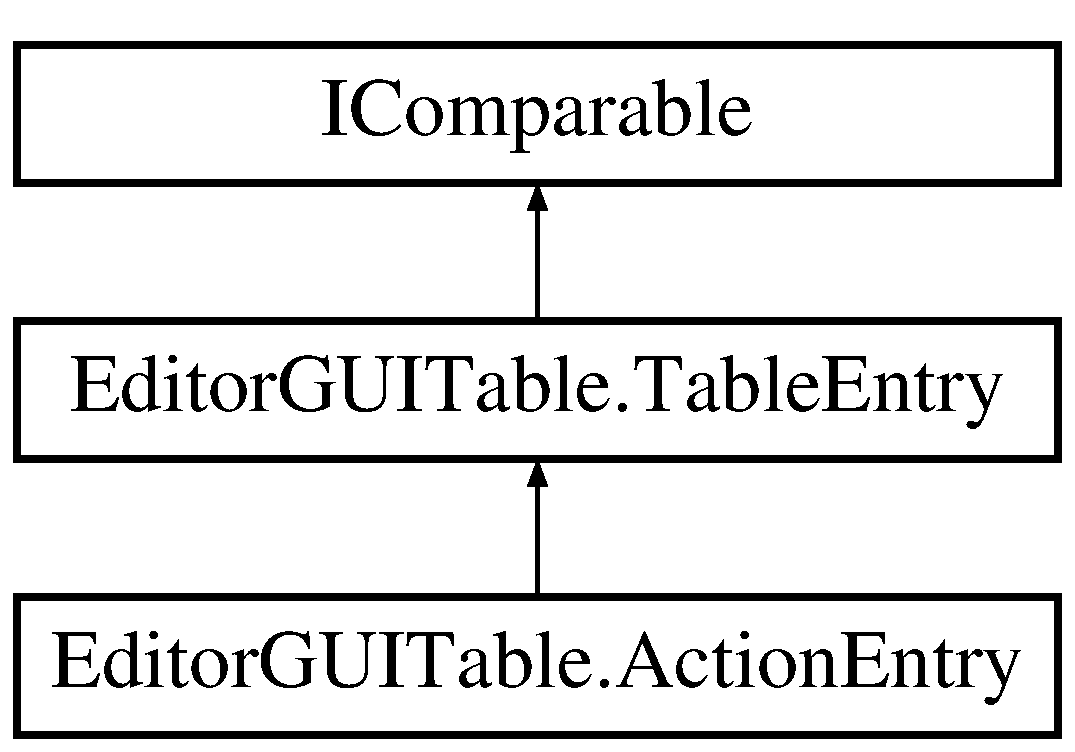
\includegraphics[height=3.000000cm]{class_editor_g_u_i_table_1_1_action_entry}
\end{center}
\end{figure}
\subsection*{Public Member Functions}
\begin{DoxyCompactItemize}
\item 
override void \mbox{\hyperlink{class_editor_g_u_i_table_1_1_action_entry_ae556137b72e1e356a2e4cf4a12b88336}{Draw\+Entry\+Layout}} (float width, float height)
\begin{DoxyCompactList}\small\item\em Draws the entry using G\+U\+I\+Layout. \end{DoxyCompactList}\item 
override void \mbox{\hyperlink{class_editor_g_u_i_table_1_1_action_entry_a84dfbc114f27c8108899c3c25803ae60}{Draw\+Entry}} (Rect rect)
\begin{DoxyCompactList}\small\item\em Draws the entry using G\+UI (without G\+U\+I\+Layout). \end{DoxyCompactList}\item 
\mbox{\Hypertarget{class_editor_g_u_i_table_1_1_action_entry_aa122ca24d9455d04facc8790c7977010}\label{class_editor_g_u_i_table_1_1_action_entry_aa122ca24d9455d04facc8790c7977010}} 
{\bfseries Action\+Entry} (string name, System.\+Action action)
\end{DoxyCompactItemize}
\subsection*{Properties}
\begin{DoxyCompactItemize}
\item 
\mbox{\Hypertarget{class_editor_g_u_i_table_1_1_action_entry_ab7ea5f66038bfda1150c35f1161b11df}\label{class_editor_g_u_i_table_1_1_action_entry_ab7ea5f66038bfda1150c35f1161b11df}} 
override string {\bfseries comparing\+Value}\hspace{0.3cm}{\ttfamily  \mbox{[}get\mbox{]}}
\end{DoxyCompactItemize}


\subsection{Detailed Description}
This entry class draws a button which, when clicked, will trigger the action given in the constructor. 



\subsection{Member Function Documentation}
\mbox{\Hypertarget{class_editor_g_u_i_table_1_1_action_entry_a84dfbc114f27c8108899c3c25803ae60}\label{class_editor_g_u_i_table_1_1_action_entry_a84dfbc114f27c8108899c3c25803ae60}} 
\index{Editor\+G\+U\+I\+Table\+::\+Action\+Entry@{Editor\+G\+U\+I\+Table\+::\+Action\+Entry}!Draw\+Entry@{Draw\+Entry}}
\index{Draw\+Entry@{Draw\+Entry}!Editor\+G\+U\+I\+Table\+::\+Action\+Entry@{Editor\+G\+U\+I\+Table\+::\+Action\+Entry}}
\subsubsection{\texorpdfstring{Draw\+Entry()}{DrawEntry()}}
{\footnotesize\ttfamily override void Editor\+G\+U\+I\+Table.\+Action\+Entry.\+Draw\+Entry (\begin{DoxyParamCaption}\item[{Rect}]{rect }\end{DoxyParamCaption})\hspace{0.3cm}{\ttfamily [inline]}, {\ttfamily [virtual]}}



Draws the entry using G\+UI (without G\+U\+I\+Layout). 


\begin{DoxyParams}{Parameters}
{\em rect} & Rect.\\
\hline
\end{DoxyParams}


Implements \mbox{\hyperlink{class_editor_g_u_i_table_1_1_table_entry_ae02e641122da6dd161d61a20576812ca}{Editor\+G\+U\+I\+Table.\+Table\+Entry}}.

\mbox{\Hypertarget{class_editor_g_u_i_table_1_1_action_entry_ae556137b72e1e356a2e4cf4a12b88336}\label{class_editor_g_u_i_table_1_1_action_entry_ae556137b72e1e356a2e4cf4a12b88336}} 
\index{Editor\+G\+U\+I\+Table\+::\+Action\+Entry@{Editor\+G\+U\+I\+Table\+::\+Action\+Entry}!Draw\+Entry\+Layout@{Draw\+Entry\+Layout}}
\index{Draw\+Entry\+Layout@{Draw\+Entry\+Layout}!Editor\+G\+U\+I\+Table\+::\+Action\+Entry@{Editor\+G\+U\+I\+Table\+::\+Action\+Entry}}
\subsubsection{\texorpdfstring{Draw\+Entry\+Layout()}{DrawEntryLayout()}}
{\footnotesize\ttfamily override void Editor\+G\+U\+I\+Table.\+Action\+Entry.\+Draw\+Entry\+Layout (\begin{DoxyParamCaption}\item[{float}]{width,  }\item[{float}]{height }\end{DoxyParamCaption})\hspace{0.3cm}{\ttfamily [inline]}, {\ttfamily [virtual]}}



Draws the entry using G\+U\+I\+Layout. 


\begin{DoxyParams}{Parameters}
{\em width} & Width.\\
\hline
{\em height} & Height.\\
\hline
\end{DoxyParams}


Implements \mbox{\hyperlink{class_editor_g_u_i_table_1_1_table_entry_abe1e2747e56d50731eeec28635b366a1}{Editor\+G\+U\+I\+Table.\+Table\+Entry}}.



The documentation for this class was generated from the following file\+:\begin{DoxyCompactItemize}
\item 
Editor/\+Entries/Action\+Entry.\+cs\end{DoxyCompactItemize}

\hypertarget{class_editor_g_u_i_table_1_1_g_u_i_table_entry}{}\section{Editor\+G\+U\+I\+Table.\+G\+U\+I\+Table\+Entry Class Reference}
\label{class_editor_g_u_i_table_1_1_g_u_i_table_entry}\index{Editor\+G\+U\+I\+Table.\+G\+U\+I\+Table\+Entry@{Editor\+G\+U\+I\+Table.\+G\+U\+I\+Table\+Entry}}
\subsection*{Public Member Functions}
\begin{DoxyCompactItemize}
\item 
\mbox{\Hypertarget{class_editor_g_u_i_table_1_1_g_u_i_table_entry_a54c8219bb9a9ffd82ee2e1d465218b6a}\label{class_editor_g_u_i_table_1_1_g_u_i_table_entry_a54c8219bb9a9ffd82ee2e1d465218b6a}} 
{\bfseries G\+U\+I\+Table\+Entry} (\mbox{\hyperlink{class_editor_g_u_i_table_1_1_g_u_i_table_option}{G\+U\+I\+Table\+Option}}\mbox{[}$\,$\mbox{]} options)
\item 
\mbox{\Hypertarget{class_editor_g_u_i_table_1_1_g_u_i_table_entry_a2cea5d7b31567e6ab2a9b7abb4199d87}\label{class_editor_g_u_i_table_1_1_g_u_i_table_entry_a2cea5d7b31567e6ab2a9b7abb4199d87}} 
virtual void {\bfseries Apply\+Options} (\mbox{\hyperlink{class_editor_g_u_i_table_1_1_g_u_i_table_option}{G\+U\+I\+Table\+Option}}\mbox{[}$\,$\mbox{]} options)
\end{DoxyCompactItemize}
\subsection*{Public Attributes}
\begin{DoxyCompactItemize}
\item 
\mbox{\Hypertarget{class_editor_g_u_i_table_1_1_g_u_i_table_entry_a05effff7e10bff686425949541c2fd3d}\label{class_editor_g_u_i_table_1_1_g_u_i_table_entry_a05effff7e10bff686425949541c2fd3d}} 
bool {\bfseries allow\+Scroll\+View} = true
\item 
\mbox{\Hypertarget{class_editor_g_u_i_table_1_1_g_u_i_table_entry_a3c4abaa7a9d84c7af19bee8ddac29f37}\label{class_editor_g_u_i_table_1_1_g_u_i_table_entry_a3c4abaa7a9d84c7af19bee8ddac29f37}} 
float {\bfseries row\+Height} = Unity\+Editor.\+Editor\+G\+U\+I\+Utility.\+single\+Line\+Height
\end{DoxyCompactItemize}


The documentation for this class was generated from the following file\+:\begin{DoxyCompactItemize}
\item 
Editor/G\+U\+I\+Table\+Entry.\+cs\end{DoxyCompactItemize}

\hypertarget{class_editor_g_u_i_table_1_1_g_u_i_table_option}{}\section{Editor\+G\+U\+I\+Table.\+G\+U\+I\+Table\+Option Class Reference}
\label{class_editor_g_u_i_table_1_1_g_u_i_table_option}\index{Editor\+G\+U\+I\+Table.\+G\+U\+I\+Table\+Option@{Editor\+G\+U\+I\+Table.\+G\+U\+I\+Table\+Option}}
\subsection*{Public Types}
\begin{DoxyCompactItemize}
\item 
\mbox{\Hypertarget{class_editor_g_u_i_table_1_1_g_u_i_table_option_a095cb87443fb1af279bfdad89fc97979}\label{class_editor_g_u_i_table_1_1_g_u_i_table_option_a095cb87443fb1af279bfdad89fc97979}} 
enum {\bfseries Type} \{ {\bfseries Allow\+Scroll\+View}, 
{\bfseries Row\+Height}
 \}
\end{DoxyCompactItemize}
\subsection*{Public Member Functions}
\begin{DoxyCompactItemize}
\item 
\mbox{\Hypertarget{class_editor_g_u_i_table_1_1_g_u_i_table_option_a985af09f31c25e1473e42d310f17ec61}\label{class_editor_g_u_i_table_1_1_g_u_i_table_option_a985af09f31c25e1473e42d310f17ec61}} 
{\bfseries G\+U\+I\+Table\+Option} (Type type, object value)
\end{DoxyCompactItemize}
\subsection*{Static Public Member Functions}
\begin{DoxyCompactItemize}
\item 
\mbox{\Hypertarget{class_editor_g_u_i_table_1_1_g_u_i_table_option_a7136ea1312738cf943f7318b9d96baff}\label{class_editor_g_u_i_table_1_1_g_u_i_table_option_a7136ea1312738cf943f7318b9d96baff}} 
static \mbox{\hyperlink{class_editor_g_u_i_table_1_1_g_u_i_table_option}{G\+U\+I\+Table\+Option}} {\bfseries Allow\+Scroll\+View} (bool enable)
\item 
\mbox{\Hypertarget{class_editor_g_u_i_table_1_1_g_u_i_table_option_a2cdf1ca2f313a150f12e08bee2e034a0}\label{class_editor_g_u_i_table_1_1_g_u_i_table_option_a2cdf1ca2f313a150f12e08bee2e034a0}} 
static \mbox{\hyperlink{class_editor_g_u_i_table_1_1_g_u_i_table_option}{G\+U\+I\+Table\+Option}} {\bfseries Row\+Height} (float value)
\end{DoxyCompactItemize}
\subsection*{Public Attributes}
\begin{DoxyCompactItemize}
\item 
\mbox{\Hypertarget{class_editor_g_u_i_table_1_1_g_u_i_table_option_aac0499445c98f69b27012f6348fb4fb3}\label{class_editor_g_u_i_table_1_1_g_u_i_table_option_aac0499445c98f69b27012f6348fb4fb3}} 
Type {\bfseries type}
\item 
\mbox{\Hypertarget{class_editor_g_u_i_table_1_1_g_u_i_table_option_a0cfad34a241e2c7c777ba82a5eeb23e2}\label{class_editor_g_u_i_table_1_1_g_u_i_table_option_a0cfad34a241e2c7c777ba82a5eeb23e2}} 
object {\bfseries value}
\end{DoxyCompactItemize}


The documentation for this class was generated from the following file\+:\begin{DoxyCompactItemize}
\item 
Editor/G\+U\+I\+Table\+Option.\+cs\end{DoxyCompactItemize}

\hypertarget{class_editor_g_u_i_table_1_1_g_u_i_table_state}{}\section{Editor\+G\+U\+I\+Table.\+G\+U\+I\+Table\+State Class Reference}
\label{class_editor_g_u_i_table_1_1_g_u_i_table_state}\index{Editor\+G\+U\+I\+Table.\+G\+U\+I\+Table\+State@{Editor\+G\+U\+I\+Table.\+G\+U\+I\+Table\+State}}


The current state of the G\+U\+I\+Table. This has to be used the same way state parameters are used in Unity G\+UI functions, like the scroll position in Begin\+Scroll\+View. It has to be passed from one G\+UI frame to another by keeping a reference in your calling code.  


\subsection*{Public Member Functions}
\begin{DoxyCompactItemize}
\item 
\mbox{\hyperlink{class_editor_g_u_i_table_1_1_g_u_i_table_state_aab7e8f3314020a2f5fda74e6d618d330}{G\+U\+I\+Table\+State}} (string prefs\+Key)
\begin{DoxyCompactList}\small\item\em Initializes a G\+U\+I\+Extensions.\+G\+U\+I\+Table\+State with a key to save it in Editor\+Prefs. This constructor can\textquotesingle{}t be used in Scriptable\+Object\textquotesingle{}s constructor or in the property\textquotesingle{}s declaration, because it uses the Editor\+Prefs. Use it in On\+Enable or Awake instead. \end{DoxyCompactList}\item 
\mbox{\Hypertarget{class_editor_g_u_i_table_1_1_g_u_i_table_state_a02acb0bb7c75ca1bcd97a2f89da2617b}\label{class_editor_g_u_i_table_1_1_g_u_i_table_state_a02acb0bb7c75ca1bcd97a2f89da2617b}} 
void {\bfseries Save} ()
\end{DoxyCompactItemize}
\subsection*{Static Public Member Functions}
\begin{DoxyCompactItemize}
\item 
\mbox{\Hypertarget{class_editor_g_u_i_table_1_1_g_u_i_table_state_afe7dda29a996965d4b42b6861a148115}\label{class_editor_g_u_i_table_1_1_g_u_i_table_state_afe7dda29a996965d4b42b6861a148115}} 
static \mbox{\hyperlink{class_editor_g_u_i_table_1_1_g_u_i_table_state}{G\+U\+I\+Table\+State}} {\bfseries Load} (string prefs\+Key)
\end{DoxyCompactItemize}
\subsection*{Public Attributes}
\begin{DoxyCompactItemize}
\item 
\mbox{\Hypertarget{class_editor_g_u_i_table_1_1_g_u_i_table_state_a5d522c1790784ff16db98b345b74a0ca}\label{class_editor_g_u_i_table_1_1_g_u_i_table_state_a5d522c1790784ff16db98b345b74a0ca}} 
Vector2 {\bfseries scroll\+Pos}
\item 
\mbox{\Hypertarget{class_editor_g_u_i_table_1_1_g_u_i_table_state_ac9aaf765fd446c9e48b17b47528f647f}\label{class_editor_g_u_i_table_1_1_g_u_i_table_state_ac9aaf765fd446c9e48b17b47528f647f}} 
Vector2 {\bfseries scroll\+Pos\+Horiz}
\item 
\mbox{\Hypertarget{class_editor_g_u_i_table_1_1_g_u_i_table_state_ad4fe2697eec54139de525bb0b87be1b3}\label{class_editor_g_u_i_table_1_1_g_u_i_table_state_ad4fe2697eec54139de525bb0b87be1b3}} 
int {\bfseries sort\+By\+Column\+Index} = -\/1
\item 
\mbox{\Hypertarget{class_editor_g_u_i_table_1_1_g_u_i_table_state_a77f82460b4a1a57c23035e404ff47346}\label{class_editor_g_u_i_table_1_1_g_u_i_table_state_a77f82460b4a1a57c23035e404ff47346}} 
bool {\bfseries sort\+Increasing}
\item 
\mbox{\Hypertarget{class_editor_g_u_i_table_1_1_g_u_i_table_state_ade1dee36083109909f4bf31bd88d995e}\label{class_editor_g_u_i_table_1_1_g_u_i_table_state_ade1dee36083109909f4bf31bd88d995e}} 
List$<$ float $>$ {\bfseries column\+Sizes} = new List$<$float$>$ ()
\item 
\mbox{\Hypertarget{class_editor_g_u_i_table_1_1_g_u_i_table_state_a5351f180498096a8da853064d8a2e4d0}\label{class_editor_g_u_i_table_1_1_g_u_i_table_state_a5351f180498096a8da853064d8a2e4d0}} 
List$<$ bool $>$ {\bfseries column\+Visible} = new List$<$bool$>$ ()
\end{DoxyCompactItemize}
\subsection*{Properties}
\begin{DoxyCompactItemize}
\item 
\mbox{\Hypertarget{class_editor_g_u_i_table_1_1_g_u_i_table_state_ad2f4887bcadfd3fcdf6e4642e5be1d80}\label{class_editor_g_u_i_table_1_1_g_u_i_table_state_ad2f4887bcadfd3fcdf6e4642e5be1d80}} 
float {\bfseries total\+Width}\hspace{0.3cm}{\ttfamily  \mbox{[}get\mbox{]}}
\end{DoxyCompactItemize}


\subsection{Detailed Description}
The current state of the G\+U\+I\+Table. This has to be used the same way state parameters are used in Unity G\+UI functions, like the scroll position in Begin\+Scroll\+View. It has to be passed from one G\+UI frame to another by keeping a reference in your calling code. 


\begin{DoxyCode}
GUITableState tableState;
\textcolor{keywordtype}{void} OnGUI ()
\{
    tableState = GUITable.DrawTable(collectionProperty, tableState);
\}
\end{DoxyCode}
 

\subsection{Constructor \& Destructor Documentation}
\mbox{\Hypertarget{class_editor_g_u_i_table_1_1_g_u_i_table_state_aab7e8f3314020a2f5fda74e6d618d330}\label{class_editor_g_u_i_table_1_1_g_u_i_table_state_aab7e8f3314020a2f5fda74e6d618d330}} 
\index{Editor\+G\+U\+I\+Table\+::\+G\+U\+I\+Table\+State@{Editor\+G\+U\+I\+Table\+::\+G\+U\+I\+Table\+State}!G\+U\+I\+Table\+State@{G\+U\+I\+Table\+State}}
\index{G\+U\+I\+Table\+State@{G\+U\+I\+Table\+State}!Editor\+G\+U\+I\+Table\+::\+G\+U\+I\+Table\+State@{Editor\+G\+U\+I\+Table\+::\+G\+U\+I\+Table\+State}}
\subsubsection{\texorpdfstring{G\+U\+I\+Table\+State()}{GUITableState()}}
{\footnotesize\ttfamily Editor\+G\+U\+I\+Table.\+G\+U\+I\+Table\+State.\+G\+U\+I\+Table\+State (\begin{DoxyParamCaption}\item[{string}]{prefs\+Key }\end{DoxyParamCaption})\hspace{0.3cm}{\ttfamily [inline]}}



Initializes a G\+U\+I\+Extensions.\+G\+U\+I\+Table\+State with a key to save it in Editor\+Prefs. This constructor can\textquotesingle{}t be used in Scriptable\+Object\textquotesingle{}s constructor or in the property\textquotesingle{}s declaration, because it uses the Editor\+Prefs. Use it in On\+Enable or Awake instead. 


\begin{DoxyParams}{Parameters}
{\em prefs\+Key} & Prefs key.\\
\hline
\end{DoxyParams}


The documentation for this class was generated from the following file\+:\begin{DoxyCompactItemize}
\item 
Editor/G\+U\+I\+Table\+State.\+cs\end{DoxyCompactItemize}

\hypertarget{class_editor_g_u_i_table_1_1_label_entry}{}\section{Editor\+G\+U\+I\+Table.\+Label\+Entry Class Reference}
\label{class_editor_g_u_i_table_1_1_label_entry}\index{Editor\+G\+U\+I\+Table.\+Label\+Entry@{Editor\+G\+U\+I\+Table.\+Label\+Entry}}


This entry class draws a string as a label. This is useful for properties you want to display in the table as read only, as the default Property\+Field used in \mbox{\hyperlink{class_editor_g_u_i_table_1_1_property_entry}{Property\+Entry}} uses editable fields.  


Inheritance diagram for Editor\+G\+U\+I\+Table.\+Label\+Entry\+:\begin{figure}[H]
\begin{center}
\leavevmode
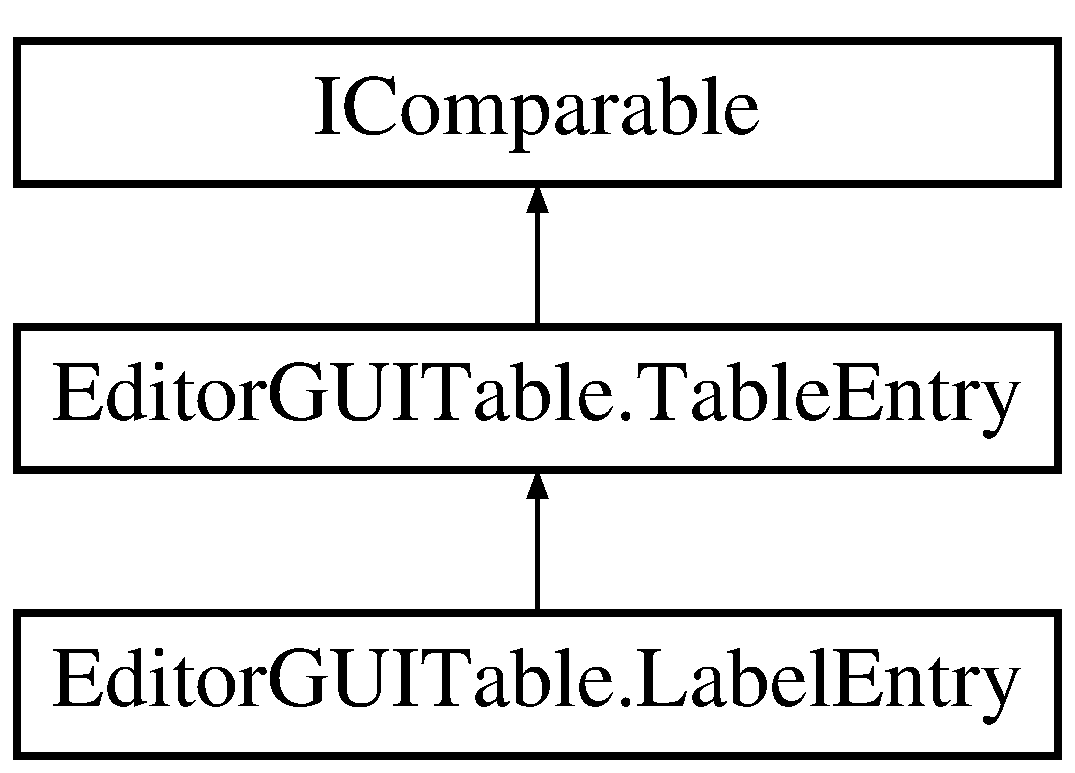
\includegraphics[height=3.000000cm]{class_editor_g_u_i_table_1_1_label_entry}
\end{center}
\end{figure}
\subsection*{Public Member Functions}
\begin{DoxyCompactItemize}
\item 
override void \mbox{\hyperlink{class_editor_g_u_i_table_1_1_label_entry_a1bf901bb1f193f4c7ff842d898968572}{Draw\+Entry\+Layout}} (float width, float height)
\begin{DoxyCompactList}\small\item\em Draws the entry using G\+U\+I\+Layout. \end{DoxyCompactList}\item 
override void \mbox{\hyperlink{class_editor_g_u_i_table_1_1_label_entry_a94247717318efb4e51347519e0b985dc}{Draw\+Entry}} (Rect rect)
\begin{DoxyCompactList}\small\item\em Draws the entry using G\+UI (without G\+U\+I\+Layout). \end{DoxyCompactList}\item 
\mbox{\Hypertarget{class_editor_g_u_i_table_1_1_label_entry_a072a6572ae589178320e873f26f883f8}\label{class_editor_g_u_i_table_1_1_label_entry_a072a6572ae589178320e873f26f883f8}} 
{\bfseries Label\+Entry} (string value)
\end{DoxyCompactItemize}
\subsection*{Properties}
\begin{DoxyCompactItemize}
\item 
\mbox{\Hypertarget{class_editor_g_u_i_table_1_1_label_entry_aea2a985feca1a1f17efefd707b67030c}\label{class_editor_g_u_i_table_1_1_label_entry_aea2a985feca1a1f17efefd707b67030c}} 
override string {\bfseries comparing\+Value}\hspace{0.3cm}{\ttfamily  \mbox{[}get\mbox{]}}
\end{DoxyCompactItemize}


\subsection{Detailed Description}
This entry class draws a string as a label. This is useful for properties you want to display in the table as read only, as the default Property\+Field used in \mbox{\hyperlink{class_editor_g_u_i_table_1_1_property_entry}{Property\+Entry}} uses editable fields. 



\subsection{Member Function Documentation}
\mbox{\Hypertarget{class_editor_g_u_i_table_1_1_label_entry_a94247717318efb4e51347519e0b985dc}\label{class_editor_g_u_i_table_1_1_label_entry_a94247717318efb4e51347519e0b985dc}} 
\index{Editor\+G\+U\+I\+Table\+::\+Label\+Entry@{Editor\+G\+U\+I\+Table\+::\+Label\+Entry}!Draw\+Entry@{Draw\+Entry}}
\index{Draw\+Entry@{Draw\+Entry}!Editor\+G\+U\+I\+Table\+::\+Label\+Entry@{Editor\+G\+U\+I\+Table\+::\+Label\+Entry}}
\subsubsection{\texorpdfstring{Draw\+Entry()}{DrawEntry()}}
{\footnotesize\ttfamily override void Editor\+G\+U\+I\+Table.\+Label\+Entry.\+Draw\+Entry (\begin{DoxyParamCaption}\item[{Rect}]{rect }\end{DoxyParamCaption})\hspace{0.3cm}{\ttfamily [inline]}, {\ttfamily [virtual]}}



Draws the entry using G\+UI (without G\+U\+I\+Layout). 


\begin{DoxyParams}{Parameters}
{\em rect} & Rect.\\
\hline
\end{DoxyParams}


Implements \mbox{\hyperlink{class_editor_g_u_i_table_1_1_table_entry_ae02e641122da6dd161d61a20576812ca}{Editor\+G\+U\+I\+Table.\+Table\+Entry}}.

\mbox{\Hypertarget{class_editor_g_u_i_table_1_1_label_entry_a1bf901bb1f193f4c7ff842d898968572}\label{class_editor_g_u_i_table_1_1_label_entry_a1bf901bb1f193f4c7ff842d898968572}} 
\index{Editor\+G\+U\+I\+Table\+::\+Label\+Entry@{Editor\+G\+U\+I\+Table\+::\+Label\+Entry}!Draw\+Entry\+Layout@{Draw\+Entry\+Layout}}
\index{Draw\+Entry\+Layout@{Draw\+Entry\+Layout}!Editor\+G\+U\+I\+Table\+::\+Label\+Entry@{Editor\+G\+U\+I\+Table\+::\+Label\+Entry}}
\subsubsection{\texorpdfstring{Draw\+Entry\+Layout()}{DrawEntryLayout()}}
{\footnotesize\ttfamily override void Editor\+G\+U\+I\+Table.\+Label\+Entry.\+Draw\+Entry\+Layout (\begin{DoxyParamCaption}\item[{float}]{width,  }\item[{float}]{height }\end{DoxyParamCaption})\hspace{0.3cm}{\ttfamily [inline]}, {\ttfamily [virtual]}}



Draws the entry using G\+U\+I\+Layout. 


\begin{DoxyParams}{Parameters}
{\em width} & Width.\\
\hline
{\em height} & Height.\\
\hline
\end{DoxyParams}


Implements \mbox{\hyperlink{class_editor_g_u_i_table_1_1_table_entry_abe1e2747e56d50731eeec28635b366a1}{Editor\+G\+U\+I\+Table.\+Table\+Entry}}.



The documentation for this class was generated from the following file\+:\begin{DoxyCompactItemize}
\item 
Editor/\+Entries/Label\+Entry.\+cs\end{DoxyCompactItemize}

\hypertarget{class_editor_g_u_i_table_1_1_property_column}{}\section{Editor\+G\+U\+I\+Table.\+Property\+Column Class Reference}
\label{class_editor_g_u_i_table_1_1_property_column}\index{Editor\+G\+U\+I\+Table.\+Property\+Column@{Editor\+G\+U\+I\+Table.\+Property\+Column}}


Internal Use Only. This class adds a property to a column. This will be used to automatically draw the entries for this column in some versions of G\+U\+I\+Table.\+Draw\+Table  


Inheritance diagram for Editor\+G\+U\+I\+Table.\+Property\+Column\+:\begin{figure}[H]
\begin{center}
\leavevmode
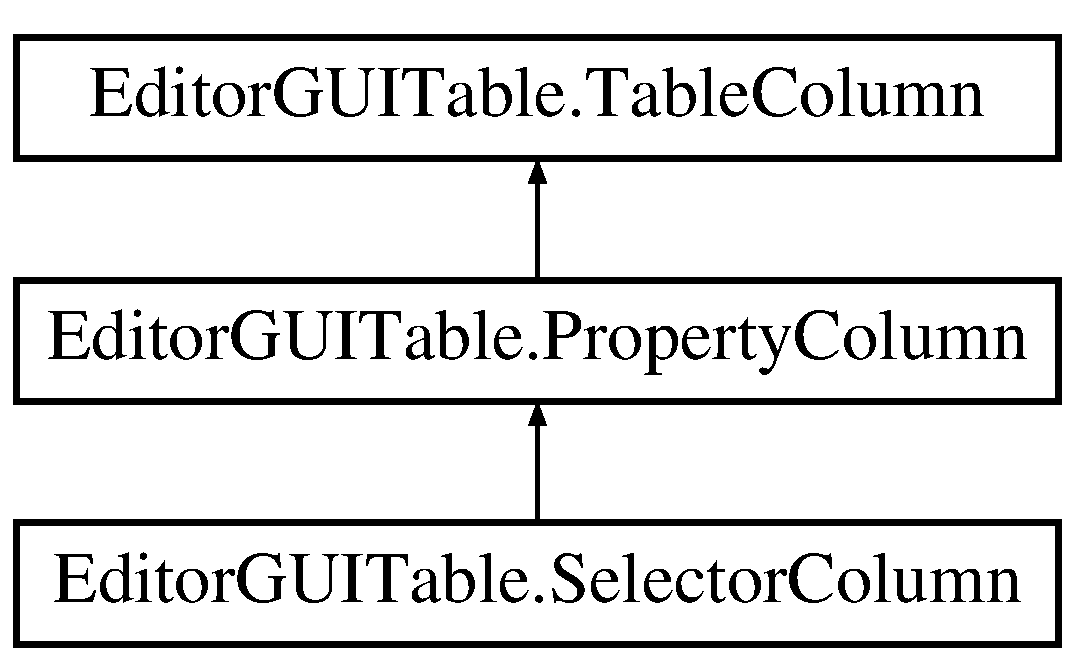
\includegraphics[height=3.000000cm]{class_editor_g_u_i_table_1_1_property_column}
\end{center}
\end{figure}
\subsection*{Public Member Functions}
\begin{DoxyCompactItemize}
\item 
\mbox{\Hypertarget{class_editor_g_u_i_table_1_1_property_column_a26dacbd8bb1ace402c8a30857cf72b0d}\label{class_editor_g_u_i_table_1_1_property_column_a26dacbd8bb1ace402c8a30857cf72b0d}} 
{\bfseries Property\+Column} (string property\+Name, string name, params \mbox{\hyperlink{class_table_column_option}{Table\+Column\+Option}}\mbox{[}$\,$\mbox{]} options)
\end{DoxyCompactItemize}
\subsection*{Public Attributes}
\begin{DoxyCompactItemize}
\item 
\mbox{\Hypertarget{class_editor_g_u_i_table_1_1_property_column_ad1b1137a273befe15ba5025ad8f4aa3e}\label{class_editor_g_u_i_table_1_1_property_column_ad1b1137a273befe15ba5025ad8f4aa3e}} 
string {\bfseries property\+Name}
\end{DoxyCompactItemize}
\subsection*{Additional Inherited Members}


\subsection{Detailed Description}
Internal Use Only. This class adds a property to a column. This will be used to automatically draw the entries for this column in some versions of G\+U\+I\+Table.\+Draw\+Table 



The documentation for this class was generated from the following file\+:\begin{DoxyCompactItemize}
\item 
Editor/\+Columns/Property\+Column.\+cs\end{DoxyCompactItemize}

\hypertarget{class_editor_g_u_i_table_1_1_property_entry}{}\section{Editor\+G\+U\+I\+Table.\+Property\+Entry Class Reference}
\label{class_editor_g_u_i_table_1_1_property_entry}\index{Editor\+G\+U\+I\+Table.\+Property\+Entry@{Editor\+G\+U\+I\+Table.\+Property\+Entry}}


This entry class just uses Editor\+G\+U\+I\+Layout.\+Property\+Field to draw a given property. This is the basic way to use G\+U\+I\+Table. It will draw the properties the same way Unity would by default.  


Inheritance diagram for Editor\+G\+U\+I\+Table.\+Property\+Entry\+:\begin{figure}[H]
\begin{center}
\leavevmode
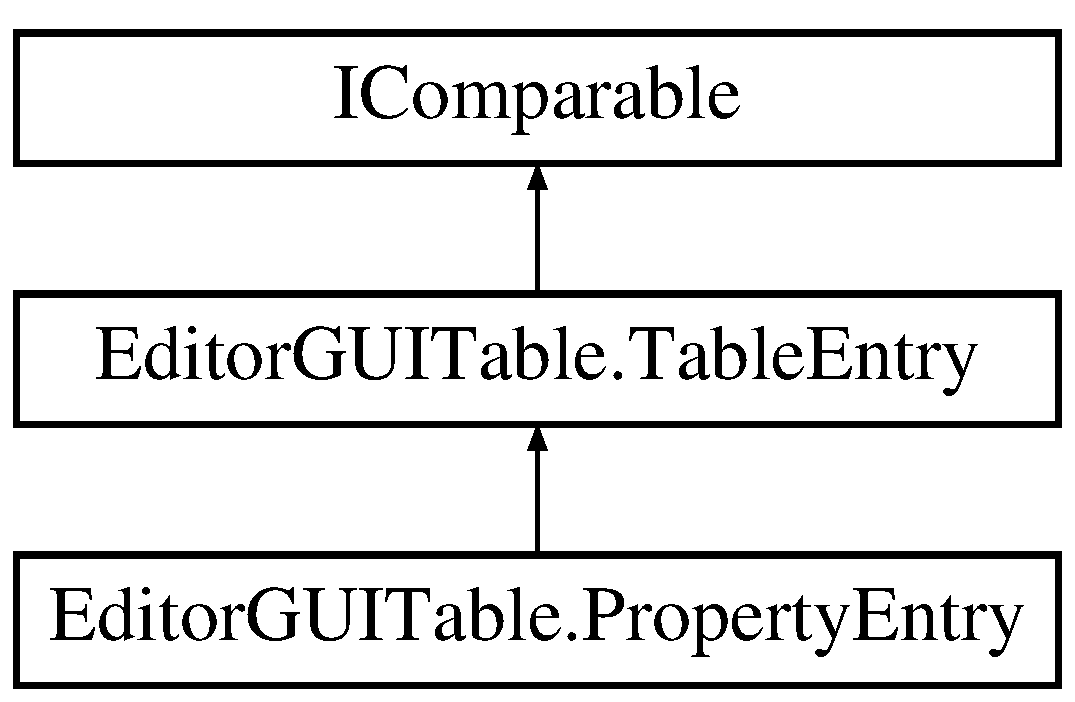
\includegraphics[height=3.000000cm]{class_editor_g_u_i_table_1_1_property_entry}
\end{center}
\end{figure}
\subsection*{Public Member Functions}
\begin{DoxyCompactItemize}
\item 
override void \mbox{\hyperlink{class_editor_g_u_i_table_1_1_property_entry_a5930e1e0e8cf4954cdbf25ef72e815f8}{Draw\+Entry\+Layout}} (float width, float height)
\begin{DoxyCompactList}\small\item\em Draws the entry using G\+U\+I\+Layout. \end{DoxyCompactList}\item 
override void \mbox{\hyperlink{class_editor_g_u_i_table_1_1_property_entry_a176094e41cb53be100106c1d58763607}{Draw\+Entry}} (Rect rect)
\begin{DoxyCompactList}\small\item\em Draws the entry using G\+UI (without G\+U\+I\+Layout). \end{DoxyCompactList}\item 
\mbox{\Hypertarget{class_editor_g_u_i_table_1_1_property_entry_a7ca61820fc62ad5de3cd974fa9740222}\label{class_editor_g_u_i_table_1_1_property_entry_a7ca61820fc62ad5de3cd974fa9740222}} 
override int {\bfseries Compare\+To} (object other)
\item 
\mbox{\Hypertarget{class_editor_g_u_i_table_1_1_property_entry_af596ccc66215ccce2b1368d14675f5e7}\label{class_editor_g_u_i_table_1_1_property_entry_af596ccc66215ccce2b1368d14675f5e7}} 
{\bfseries Property\+Entry} (Serialized\+Property property)
\item 
\mbox{\Hypertarget{class_editor_g_u_i_table_1_1_property_entry_ac45cada48f9079257cc50efbbdaec6a2}\label{class_editor_g_u_i_table_1_1_property_entry_ac45cada48f9079257cc50efbbdaec6a2}} 
{\bfseries Property\+Entry} (Serialized\+Object so, string property\+Path)
\end{DoxyCompactItemize}
\subsection*{Properties}
\begin{DoxyCompactItemize}
\item 
\mbox{\Hypertarget{class_editor_g_u_i_table_1_1_property_entry_aa8cdc61d8dc7838c7f34af454108b52c}\label{class_editor_g_u_i_table_1_1_property_entry_aa8cdc61d8dc7838c7f34af454108b52c}} 
override string {\bfseries comparing\+Value}\hspace{0.3cm}{\ttfamily  \mbox{[}get\mbox{]}}
\end{DoxyCompactItemize}


\subsection{Detailed Description}
This entry class just uses Editor\+G\+U\+I\+Layout.\+Property\+Field to draw a given property. This is the basic way to use G\+U\+I\+Table. It will draw the properties the same way Unity would by default. 



\subsection{Member Function Documentation}
\mbox{\Hypertarget{class_editor_g_u_i_table_1_1_property_entry_a176094e41cb53be100106c1d58763607}\label{class_editor_g_u_i_table_1_1_property_entry_a176094e41cb53be100106c1d58763607}} 
\index{Editor\+G\+U\+I\+Table\+::\+Property\+Entry@{Editor\+G\+U\+I\+Table\+::\+Property\+Entry}!Draw\+Entry@{Draw\+Entry}}
\index{Draw\+Entry@{Draw\+Entry}!Editor\+G\+U\+I\+Table\+::\+Property\+Entry@{Editor\+G\+U\+I\+Table\+::\+Property\+Entry}}
\subsubsection{\texorpdfstring{Draw\+Entry()}{DrawEntry()}}
{\footnotesize\ttfamily override void Editor\+G\+U\+I\+Table.\+Property\+Entry.\+Draw\+Entry (\begin{DoxyParamCaption}\item[{Rect}]{rect }\end{DoxyParamCaption})\hspace{0.3cm}{\ttfamily [inline]}, {\ttfamily [virtual]}}



Draws the entry using G\+UI (without G\+U\+I\+Layout). 


\begin{DoxyParams}{Parameters}
{\em rect} & Rect.\\
\hline
\end{DoxyParams}


Implements \mbox{\hyperlink{class_editor_g_u_i_table_1_1_table_entry_ae02e641122da6dd161d61a20576812ca}{Editor\+G\+U\+I\+Table.\+Table\+Entry}}.

\mbox{\Hypertarget{class_editor_g_u_i_table_1_1_property_entry_a5930e1e0e8cf4954cdbf25ef72e815f8}\label{class_editor_g_u_i_table_1_1_property_entry_a5930e1e0e8cf4954cdbf25ef72e815f8}} 
\index{Editor\+G\+U\+I\+Table\+::\+Property\+Entry@{Editor\+G\+U\+I\+Table\+::\+Property\+Entry}!Draw\+Entry\+Layout@{Draw\+Entry\+Layout}}
\index{Draw\+Entry\+Layout@{Draw\+Entry\+Layout}!Editor\+G\+U\+I\+Table\+::\+Property\+Entry@{Editor\+G\+U\+I\+Table\+::\+Property\+Entry}}
\subsubsection{\texorpdfstring{Draw\+Entry\+Layout()}{DrawEntryLayout()}}
{\footnotesize\ttfamily override void Editor\+G\+U\+I\+Table.\+Property\+Entry.\+Draw\+Entry\+Layout (\begin{DoxyParamCaption}\item[{float}]{width,  }\item[{float}]{height }\end{DoxyParamCaption})\hspace{0.3cm}{\ttfamily [inline]}, {\ttfamily [virtual]}}



Draws the entry using G\+U\+I\+Layout. 


\begin{DoxyParams}{Parameters}
{\em width} & Width.\\
\hline
{\em height} & Height.\\
\hline
\end{DoxyParams}


Implements \mbox{\hyperlink{class_editor_g_u_i_table_1_1_table_entry_abe1e2747e56d50731eeec28635b366a1}{Editor\+G\+U\+I\+Table.\+Table\+Entry}}.



The documentation for this class was generated from the following file\+:\begin{DoxyCompactItemize}
\item 
Editor/\+Entries/Property\+Entry.\+cs\end{DoxyCompactItemize}

\hypertarget{class_editor_g_u_i_table_1_1_selector_column}{}\section{Editor\+G\+U\+I\+Table.\+Selector\+Column Class Reference}
\label{class_editor_g_u_i_table_1_1_selector_column}\index{Editor\+G\+U\+I\+Table.\+Selector\+Column@{Editor\+G\+U\+I\+Table.\+Selector\+Column}}


This class adds a property and a selector to a column. This will be used to automatically draw the entries for this column in some versions of G\+U\+I\+Table.\+Draw\+Table  


Inheritance diagram for Editor\+G\+U\+I\+Table.\+Selector\+Column\+:\begin{figure}[H]
\begin{center}
\leavevmode
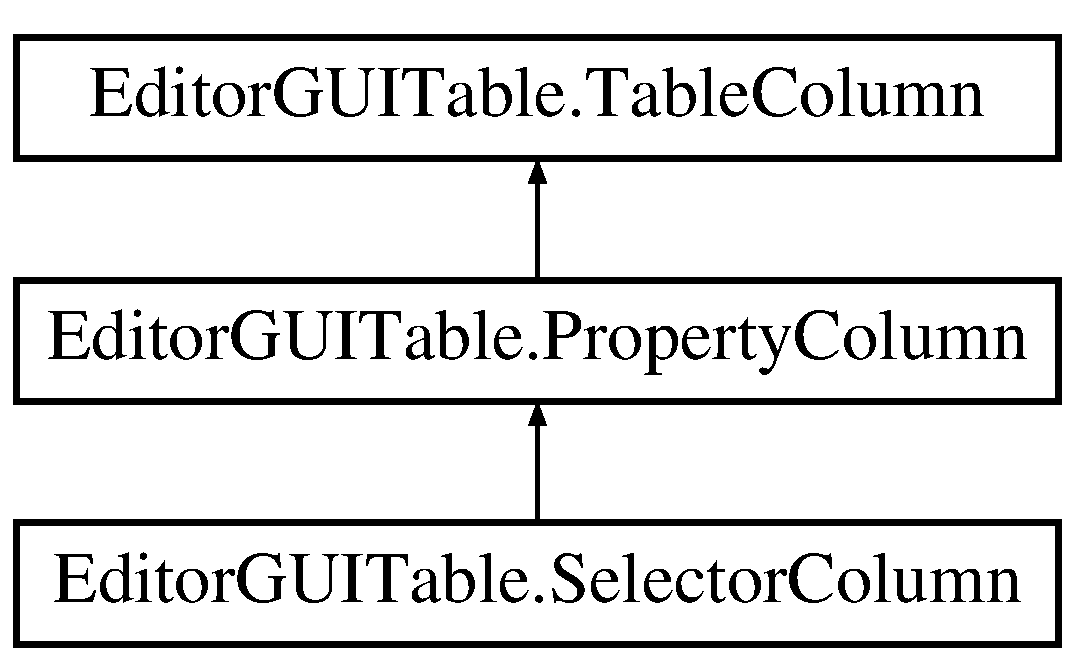
\includegraphics[height=3.000000cm]{class_editor_g_u_i_table_1_1_selector_column}
\end{center}
\end{figure}
\subsection*{Public Member Functions}
\begin{DoxyCompactItemize}
\item 
\mbox{\Hypertarget{class_editor_g_u_i_table_1_1_selector_column_a86905f52829303fc2322dc71a362941e}\label{class_editor_g_u_i_table_1_1_selector_column_a86905f52829303fc2322dc71a362941e}} 
{\bfseries Selector\+Column} (Func$<$ Serialized\+Property, \mbox{\hyperlink{class_editor_g_u_i_table_1_1_table_entry}{Table\+Entry}} $>$ selector, string property\+Name, string name, params \mbox{\hyperlink{class_table_column_option}{Table\+Column\+Option}}\mbox{[}$\,$\mbox{]} options)
\end{DoxyCompactItemize}
\subsection*{Public Attributes}
\begin{DoxyCompactItemize}
\item 
\mbox{\Hypertarget{class_editor_g_u_i_table_1_1_selector_column_a5c4dffe1ceb563f968a0041b0d433ec6}\label{class_editor_g_u_i_table_1_1_selector_column_a5c4dffe1ceb563f968a0041b0d433ec6}} 
Func$<$ Serialized\+Property, \mbox{\hyperlink{class_editor_g_u_i_table_1_1_table_entry}{Table\+Entry}} $>$ {\bfseries selector}
\end{DoxyCompactItemize}
\subsection*{Additional Inherited Members}


\subsection{Detailed Description}
This class adds a property and a selector to a column. This will be used to automatically draw the entries for this column in some versions of G\+U\+I\+Table.\+Draw\+Table 



The documentation for this class was generated from the following file\+:\begin{DoxyCompactItemize}
\item 
Editor/\+Columns/Selector\+Column.\+cs\end{DoxyCompactItemize}

\hypertarget{class_editor_g_u_i_table_1_1_table_column}{}\section{Editor\+G\+U\+I\+Table.\+Table\+Column Class Reference}
\label{class_editor_g_u_i_table_1_1_table_column}\index{Editor\+G\+U\+I\+Table.\+Table\+Column@{Editor\+G\+U\+I\+Table.\+Table\+Column}}


Base class for all table columns. It only takes a title and a width in the constructor, but other settings are available to customize the column.  


Inheritance diagram for Editor\+G\+U\+I\+Table.\+Table\+Column\+:\begin{figure}[H]
\begin{center}
\leavevmode
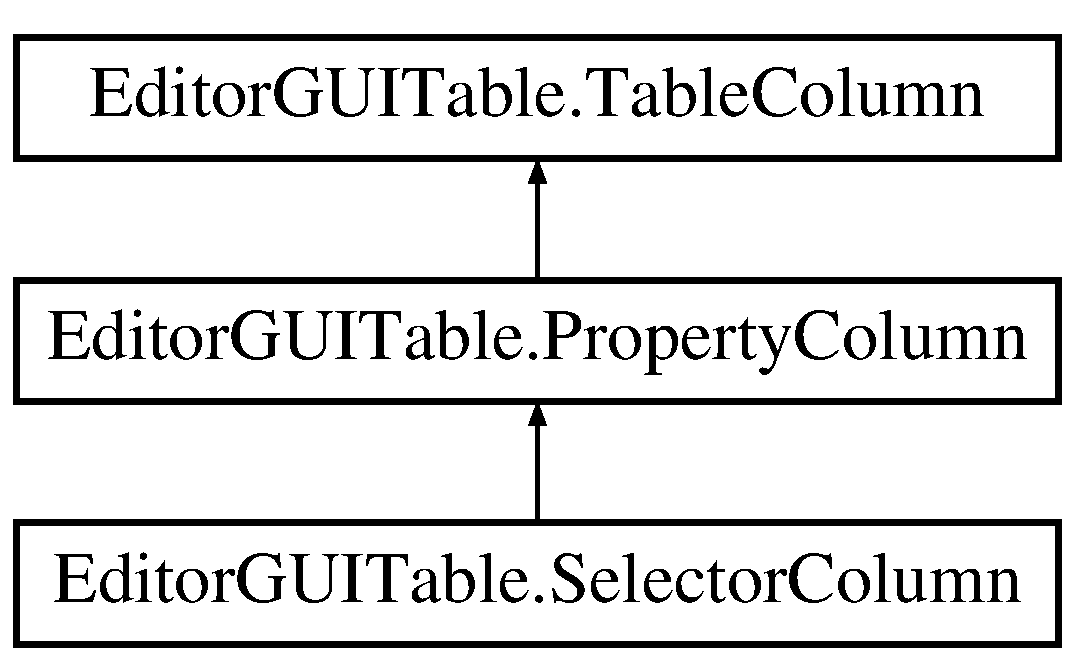
\includegraphics[height=3.000000cm]{class_editor_g_u_i_table_1_1_table_column}
\end{center}
\end{figure}
\subsection*{Public Member Functions}
\begin{DoxyCompactItemize}
\item 
\mbox{\hyperlink{class_editor_g_u_i_table_1_1_table_column_adfb68a7994e1329ac769c79d9d5c332d}{Table\+Column}} (string title, params \mbox{\hyperlink{class_table_column_option}{Table\+Column\+Option}}\mbox{[}$\,$\mbox{]} options)
\begin{DoxyCompactList}\small\item\em Initializes a column with its title and options. Edit the other public properties for more settings. \end{DoxyCompactList}\item 
\mbox{\Hypertarget{class_editor_g_u_i_table_1_1_table_column_a63ad9fb2478afb63febf24e9ed4d5890}\label{class_editor_g_u_i_table_1_1_table_column_a63ad9fb2478afb63febf24e9ed4d5890}} 
{\bfseries Table\+Column} (string title, float width)
\end{DoxyCompactItemize}
\subsection*{Static Public Member Functions}
\begin{DoxyCompactItemize}
\item 
\mbox{\Hypertarget{class_editor_g_u_i_table_1_1_table_column_a09da3ea97c951019a94b0b5123146e7b}\label{class_editor_g_u_i_table_1_1_table_column_a09da3ea97c951019a94b0b5123146e7b}} 
static \mbox{\hyperlink{class_table_column_option}{Table\+Column\+Option}} {\bfseries Expand\+Width} (bool enable)
\item 
\mbox{\Hypertarget{class_editor_g_u_i_table_1_1_table_column_a768aecae0a16bd4d69692dfd6a40c809}\label{class_editor_g_u_i_table_1_1_table_column_a768aecae0a16bd4d69692dfd6a40c809}} 
static \mbox{\hyperlink{class_table_column_option}{Table\+Column\+Option}} {\bfseries Min\+Width} (float value)
\item 
\mbox{\Hypertarget{class_editor_g_u_i_table_1_1_table_column_a4e03c2abfdcb3d3873408de863b5d84a}\label{class_editor_g_u_i_table_1_1_table_column_a4e03c2abfdcb3d3873408de863b5d84a}} 
static \mbox{\hyperlink{class_table_column_option}{Table\+Column\+Option}} {\bfseries Max\+Width} (float value)
\item 
\mbox{\Hypertarget{class_editor_g_u_i_table_1_1_table_column_a131c2c51b8487b35708c14756bc56159}\label{class_editor_g_u_i_table_1_1_table_column_a131c2c51b8487b35708c14756bc56159}} 
static \mbox{\hyperlink{class_table_column_option}{Table\+Column\+Option}} {\bfseries Width} (float value)
\item 
\mbox{\Hypertarget{class_editor_g_u_i_table_1_1_table_column_af4ed3ca6afa30ccb5d1da776b37b21e6}\label{class_editor_g_u_i_table_1_1_table_column_af4ed3ca6afa30ccb5d1da776b37b21e6}} 
static \mbox{\hyperlink{class_table_column_option}{Table\+Column\+Option}} {\bfseries Resizeable} (bool value)
\item 
\mbox{\Hypertarget{class_editor_g_u_i_table_1_1_table_column_adbaa9dd67cf167506217279715b646e4}\label{class_editor_g_u_i_table_1_1_table_column_adbaa9dd67cf167506217279715b646e4}} 
static \mbox{\hyperlink{class_table_column_option}{Table\+Column\+Option}} {\bfseries Sortable} (bool value)
\item 
\mbox{\Hypertarget{class_editor_g_u_i_table_1_1_table_column_a75178ce2e3d7ad11758d413968b1fb66}\label{class_editor_g_u_i_table_1_1_table_column_a75178ce2e3d7ad11758d413968b1fb66}} 
static \mbox{\hyperlink{class_table_column_option}{Table\+Column\+Option}} {\bfseries Enabled\+Title} (bool value)
\item 
\mbox{\Hypertarget{class_editor_g_u_i_table_1_1_table_column_a86d1eda120806f1b74c25e01debcd65e}\label{class_editor_g_u_i_table_1_1_table_column_a86d1eda120806f1b74c25e01debcd65e}} 
static \mbox{\hyperlink{class_table_column_option}{Table\+Column\+Option}} {\bfseries Enabled\+Entries} (bool value)
\item 
\mbox{\Hypertarget{class_editor_g_u_i_table_1_1_table_column_ade101144654dfd6c42c5da8b3aa4f633}\label{class_editor_g_u_i_table_1_1_table_column_ade101144654dfd6c42c5da8b3aa4f633}} 
static \mbox{\hyperlink{class_table_column_option}{Table\+Column\+Option}} {\bfseries Optional} (bool value)
\item 
\mbox{\Hypertarget{class_editor_g_u_i_table_1_1_table_column_ad19a110c1ba8ba032a0fa8456afd2e2c}\label{class_editor_g_u_i_table_1_1_table_column_ad19a110c1ba8ba032a0fa8456afd2e2c}} 
static \mbox{\hyperlink{class_table_column_option}{Table\+Column\+Option}} {\bfseries Visible\+By\+Default} (bool value)
\end{DoxyCompactItemize}
\subsection*{Public Attributes}
\begin{DoxyCompactItemize}
\item 
\mbox{\Hypertarget{class_editor_g_u_i_table_1_1_table_column_a8b0dc515475070913d584c9497007d9b}\label{class_editor_g_u_i_table_1_1_table_column_a8b0dc515475070913d584c9497007d9b}} 
\mbox{\hyperlink{class_table_column_entry}{Table\+Column\+Entry}} {\bfseries entry}
\end{DoxyCompactItemize}
\subsection*{Properties}
\begin{DoxyCompactItemize}
\item 
\mbox{\Hypertarget{class_editor_g_u_i_table_1_1_table_column_a8f7eb4ab0c9a938d772953fc4c78b9af}\label{class_editor_g_u_i_table_1_1_table_column_a8f7eb4ab0c9a938d772953fc4c78b9af}} 
string {\bfseries title}\hspace{0.3cm}{\ttfamily  \mbox{[}get\mbox{]}}
\end{DoxyCompactItemize}


\subsection{Detailed Description}
Base class for all table columns. It only takes a title and a width in the constructor, but other settings are available to customize the column. 



\subsection{Constructor \& Destructor Documentation}
\mbox{\Hypertarget{class_editor_g_u_i_table_1_1_table_column_adfb68a7994e1329ac769c79d9d5c332d}\label{class_editor_g_u_i_table_1_1_table_column_adfb68a7994e1329ac769c79d9d5c332d}} 
\index{Editor\+G\+U\+I\+Table\+::\+Table\+Column@{Editor\+G\+U\+I\+Table\+::\+Table\+Column}!Table\+Column@{Table\+Column}}
\index{Table\+Column@{Table\+Column}!Editor\+G\+U\+I\+Table\+::\+Table\+Column@{Editor\+G\+U\+I\+Table\+::\+Table\+Column}}
\subsubsection{\texorpdfstring{Table\+Column()}{TableColumn()}}
{\footnotesize\ttfamily Editor\+G\+U\+I\+Table.\+Table\+Column.\+Table\+Column (\begin{DoxyParamCaption}\item[{string}]{title,  }\item[{params \mbox{\hyperlink{class_table_column_option}{Table\+Column\+Option}} \mbox{[}$\,$\mbox{]}}]{options }\end{DoxyParamCaption})\hspace{0.3cm}{\ttfamily [inline]}}



Initializes a column with its title and options. Edit the other public properties for more settings. 


\begin{DoxyParams}{Parameters}
{\em title} & The column title.\\
\hline
{\em options} & The column options.\\
\hline
\end{DoxyParams}


The documentation for this class was generated from the following file\+:\begin{DoxyCompactItemize}
\item 
Editor/\+Columns/Table\+Column.\+cs\end{DoxyCompactItemize}

\hypertarget{class_table_column_entry}{}\section{Table\+Column\+Entry Class Reference}
\label{class_table_column_entry}\index{Table\+Column\+Entry@{Table\+Column\+Entry}}
\subsection*{Public Member Functions}
\begin{DoxyCompactItemize}
\item 
\mbox{\hyperlink{class_table_column_entry_af655798cdcaa427f57b1065e54afbc71}{Table\+Column\+Entry}} (\mbox{\hyperlink{class_table_column_option}{Table\+Column\+Option}}\mbox{[}$\,$\mbox{]} options)
\begin{DoxyCompactList}\small\item\em Defines if the column is expandable. \end{DoxyCompactList}\item 
\mbox{\Hypertarget{class_table_column_entry_add3ff00a26e27b2d94df48b9c6fade1a}\label{class_table_column_entry_add3ff00a26e27b2d94df48b9c6fade1a}} 
virtual void {\bfseries Apply\+Options} (\mbox{\hyperlink{class_table_column_option}{Table\+Column\+Option}}\mbox{[}$\,$\mbox{]} options)
\end{DoxyCompactItemize}
\subsection*{Public Attributes}
\begin{DoxyCompactItemize}
\item 
\mbox{\Hypertarget{class_table_column_entry_a08139cc094136d8c57b12fd6b95b31de}\label{class_table_column_entry_a08139cc094136d8c57b12fd6b95b31de}} 
float {\bfseries default\+Width} = 100f
\item 
\mbox{\Hypertarget{class_table_column_entry_a77f73236638c69a797520dd45a72909f}\label{class_table_column_entry_a77f73236638c69a797520dd45a72909f}} 
bool {\bfseries expand\+Width} = false
\item 
\mbox{\Hypertarget{class_table_column_entry_ae173513141ac9b369aeda1a505f71037}\label{class_table_column_entry_ae173513141ac9b369aeda1a505f71037}} 
float {\bfseries max\+Width} = float.\+Max\+Value
\item 
\mbox{\Hypertarget{class_table_column_entry_a042c46023ba0ecda8ab5dc09a583f1b8}\label{class_table_column_entry_a042c46023ba0ecda8ab5dc09a583f1b8}} 
float {\bfseries min\+Width} = 20f
\item 
\mbox{\Hypertarget{class_table_column_entry_a1512e062e4fc3b3cfdc134a2a984acc0}\label{class_table_column_entry_a1512e062e4fc3b3cfdc134a2a984acc0}} 
bool {\bfseries resizeable} = true
\item 
\mbox{\Hypertarget{class_table_column_entry_ae6cfc37ad06ec5a1014b7ad2de6152c5}\label{class_table_column_entry_ae6cfc37ad06ec5a1014b7ad2de6152c5}} 
bool {\bfseries sortable} = true
\item 
bool \mbox{\hyperlink{class_table_column_entry_a67b708efeb53404a92acd14d3d835be5}{enabled\+Entries}} = true
\begin{DoxyCompactList}\small\item\em Defines if the entries are enabled (interactable) or disabled (grayed out). Default\+: true. \end{DoxyCompactList}\item 
bool \mbox{\hyperlink{class_table_column_entry_ac15f6f79fd208e7d3cf25d38e94c2b24}{is\+Sortable}} = true
\begin{DoxyCompactList}\small\item\em Defines if the column is sortable. \end{DoxyCompactList}\item 
bool \mbox{\hyperlink{class_table_column_entry_ad861d6d58bae1518e32a3a9351effbb7}{enabled\+Title}} = true
\begin{DoxyCompactList}\small\item\em Defines if the title is enabled (interactable) or disabled (grayed out). Default\+: true. \end{DoxyCompactList}\item 
bool \mbox{\hyperlink{class_table_column_entry_a475870b7af204554a3ee617cc68886e1}{optional}} = false
\begin{DoxyCompactList}\small\item\em Defines if the column can be hidden by right-\/clicking the column titles bar. Default\+: false. \end{DoxyCompactList}\item 
bool \mbox{\hyperlink{class_table_column_entry_a4271193e2502ef06798966773677d3a8}{visible\+By\+Default}} = true
\begin{DoxyCompactList}\small\item\em Defines if the column is visible by default. If this is false, and optional is false too. The column can never be viewed. Default\+: true. \end{DoxyCompactList}\end{DoxyCompactItemize}


\subsection{Constructor \& Destructor Documentation}
\mbox{\Hypertarget{class_table_column_entry_af655798cdcaa427f57b1065e54afbc71}\label{class_table_column_entry_af655798cdcaa427f57b1065e54afbc71}} 
\index{Table\+Column\+Entry@{Table\+Column\+Entry}!Table\+Column\+Entry@{Table\+Column\+Entry}}
\index{Table\+Column\+Entry@{Table\+Column\+Entry}!Table\+Column\+Entry@{Table\+Column\+Entry}}
\subsubsection{\texorpdfstring{Table\+Column\+Entry()}{TableColumnEntry()}}
{\footnotesize\ttfamily Table\+Column\+Entry.\+Table\+Column\+Entry (\begin{DoxyParamCaption}\item[{\mbox{\hyperlink{class_table_column_option}{Table\+Column\+Option}} \mbox{[}$\,$\mbox{]}}]{options }\end{DoxyParamCaption})\hspace{0.3cm}{\ttfamily [inline]}}



Defines if the column is expandable. 



\subsection{Member Data Documentation}
\mbox{\Hypertarget{class_table_column_entry_a67b708efeb53404a92acd14d3d835be5}\label{class_table_column_entry_a67b708efeb53404a92acd14d3d835be5}} 
\index{Table\+Column\+Entry@{Table\+Column\+Entry}!enabled\+Entries@{enabled\+Entries}}
\index{enabled\+Entries@{enabled\+Entries}!Table\+Column\+Entry@{Table\+Column\+Entry}}
\subsubsection{\texorpdfstring{enabled\+Entries}{enabledEntries}}
{\footnotesize\ttfamily bool Table\+Column\+Entry.\+enabled\+Entries = true}



Defines if the entries are enabled (interactable) or disabled (grayed out). Default\+: true. 

\mbox{\Hypertarget{class_table_column_entry_ad861d6d58bae1518e32a3a9351effbb7}\label{class_table_column_entry_ad861d6d58bae1518e32a3a9351effbb7}} 
\index{Table\+Column\+Entry@{Table\+Column\+Entry}!enabled\+Title@{enabled\+Title}}
\index{enabled\+Title@{enabled\+Title}!Table\+Column\+Entry@{Table\+Column\+Entry}}
\subsubsection{\texorpdfstring{enabled\+Title}{enabledTitle}}
{\footnotesize\ttfamily bool Table\+Column\+Entry.\+enabled\+Title = true}



Defines if the title is enabled (interactable) or disabled (grayed out). Default\+: true. 

\mbox{\Hypertarget{class_table_column_entry_ac15f6f79fd208e7d3cf25d38e94c2b24}\label{class_table_column_entry_ac15f6f79fd208e7d3cf25d38e94c2b24}} 
\index{Table\+Column\+Entry@{Table\+Column\+Entry}!is\+Sortable@{is\+Sortable}}
\index{is\+Sortable@{is\+Sortable}!Table\+Column\+Entry@{Table\+Column\+Entry}}
\subsubsection{\texorpdfstring{is\+Sortable}{isSortable}}
{\footnotesize\ttfamily bool Table\+Column\+Entry.\+is\+Sortable = true}



Defines if the column is sortable. 

\mbox{\Hypertarget{class_table_column_entry_a475870b7af204554a3ee617cc68886e1}\label{class_table_column_entry_a475870b7af204554a3ee617cc68886e1}} 
\index{Table\+Column\+Entry@{Table\+Column\+Entry}!optional@{optional}}
\index{optional@{optional}!Table\+Column\+Entry@{Table\+Column\+Entry}}
\subsubsection{\texorpdfstring{optional}{optional}}
{\footnotesize\ttfamily bool Table\+Column\+Entry.\+optional = false}



Defines if the column can be hidden by right-\/clicking the column titles bar. Default\+: false. 

\mbox{\Hypertarget{class_table_column_entry_a4271193e2502ef06798966773677d3a8}\label{class_table_column_entry_a4271193e2502ef06798966773677d3a8}} 
\index{Table\+Column\+Entry@{Table\+Column\+Entry}!visible\+By\+Default@{visible\+By\+Default}}
\index{visible\+By\+Default@{visible\+By\+Default}!Table\+Column\+Entry@{Table\+Column\+Entry}}
\subsubsection{\texorpdfstring{visible\+By\+Default}{visibleByDefault}}
{\footnotesize\ttfamily bool Table\+Column\+Entry.\+visible\+By\+Default = true}



Defines if the column is visible by default. If this is false, and optional is false too. The column can never be viewed. Default\+: true. 



The documentation for this class was generated from the following file\+:\begin{DoxyCompactItemize}
\item 
Editor/\+Columns/Table\+Column\+Entry.\+cs\end{DoxyCompactItemize}

\hypertarget{class_table_column_option}{}\section{Table\+Column\+Option Class Reference}
\label{class_table_column_option}\index{Table\+Column\+Option@{Table\+Column\+Option}}
\subsection*{Public Types}
\begin{DoxyCompactItemize}
\item 
\mbox{\Hypertarget{class_table_column_option_abf345bf5e5f731d15fc65f293b216771}\label{class_table_column_option_abf345bf5e5f731d15fc65f293b216771}} 
enum {\bfseries Type} \{ \newline
{\bfseries Expand\+Width}, 
{\bfseries Width}, 
{\bfseries Min\+Width}, 
{\bfseries Max\+Width}, 
\newline
{\bfseries Resizeable}, 
{\bfseries Sortable}, 
{\bfseries Enabled\+Entries}, 
{\bfseries Enabled\+Title}, 
\newline
{\bfseries Optional}, 
{\bfseries Visible\+By\+Default}
 \}
\end{DoxyCompactItemize}
\subsection*{Public Member Functions}
\begin{DoxyCompactItemize}
\item 
\mbox{\Hypertarget{class_table_column_option_a5f4b1c640debbbeab7c3d82ce3a5121c}\label{class_table_column_option_a5f4b1c640debbbeab7c3d82ce3a5121c}} 
{\bfseries Table\+Column\+Option} (Type type, object value)
\end{DoxyCompactItemize}
\subsection*{Public Attributes}
\begin{DoxyCompactItemize}
\item 
\mbox{\Hypertarget{class_table_column_option_a973f227204e417026b25ed7701caf2dd}\label{class_table_column_option_a973f227204e417026b25ed7701caf2dd}} 
Type {\bfseries type}
\item 
\mbox{\Hypertarget{class_table_column_option_ae6647b311841ac2884737b6825fdd7bb}\label{class_table_column_option_ae6647b311841ac2884737b6825fdd7bb}} 
object {\bfseries value}
\end{DoxyCompactItemize}


The documentation for this class was generated from the following file\+:\begin{DoxyCompactItemize}
\item 
Editor/\+Columns/Table\+Column\+Option.\+cs\end{DoxyCompactItemize}

\hypertarget{class_table_drawer}{}\section{Table\+Drawer Class Reference}
\label{class_table_drawer}\index{Table\+Drawer@{Table\+Drawer}}


Drawer for the Table Attribute. See the Table\+Attribute class documentation for the limitations of this attribute.  


Inheritance diagram for Table\+Drawer\+:\begin{figure}[H]
\begin{center}
\leavevmode
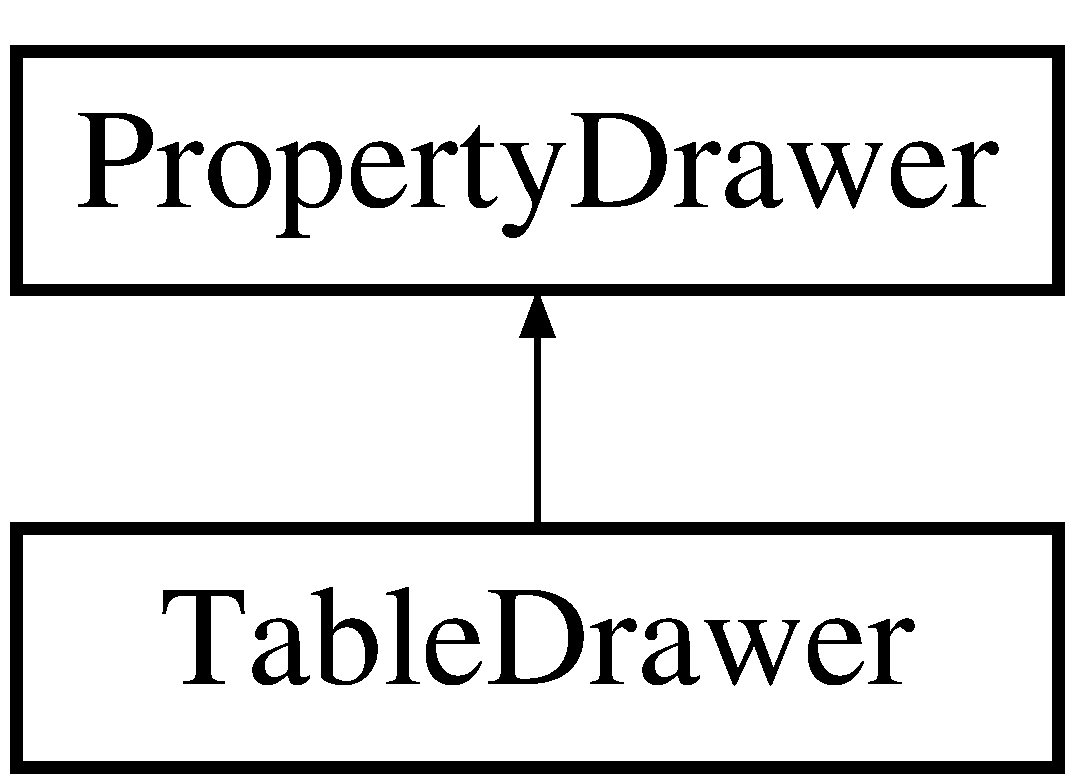
\includegraphics[height=2.000000cm]{class_table_drawer}
\end{center}
\end{figure}
\subsection*{Public Member Functions}
\begin{DoxyCompactItemize}
\item 
\mbox{\Hypertarget{class_table_drawer_a55a2658e4bff391c17b81437bcccd4c7}\label{class_table_drawer_a55a2658e4bff391c17b81437bcccd4c7}} 
override float {\bfseries Get\+Property\+Height} (Serialized\+Property property, G\+U\+I\+Content label)
\item 
\mbox{\Hypertarget{class_table_drawer_a48e0473a511f4aefef385cdf16c53839}\label{class_table_drawer_a48e0473a511f4aefef385cdf16c53839}} 
override void {\bfseries On\+G\+UI} (Rect position, Serialized\+Property property, G\+U\+I\+Content label)
\end{DoxyCompactItemize}


\subsection{Detailed Description}
Drawer for the Table Attribute. See the Table\+Attribute class documentation for the limitations of this attribute. 



The documentation for this class was generated from the following file\+:\begin{DoxyCompactItemize}
\item 
Editor/Table\+Drawer.\+cs\end{DoxyCompactItemize}

\hypertarget{class_editor_g_u_i_table_1_1_table_entry}{}\section{Editor\+G\+U\+I\+Table.\+Table\+Entry Class Reference}
\label{class_editor_g_u_i_table_1_1_table_entry}\index{Editor\+G\+U\+I\+Table.\+Table\+Entry@{Editor\+G\+U\+I\+Table.\+Table\+Entry}}


Base class for all table entries. Draw\+Entry needs to be overriden to draw the entry for the cell. Use this to customize the table however needed. Compare\+To can be overriden to customize the sorting. comparing\+Value is used as a fallback for sorting any types of entries, even different types.  


Inheritance diagram for Editor\+G\+U\+I\+Table.\+Table\+Entry\+:\begin{figure}[H]
\begin{center}
\leavevmode
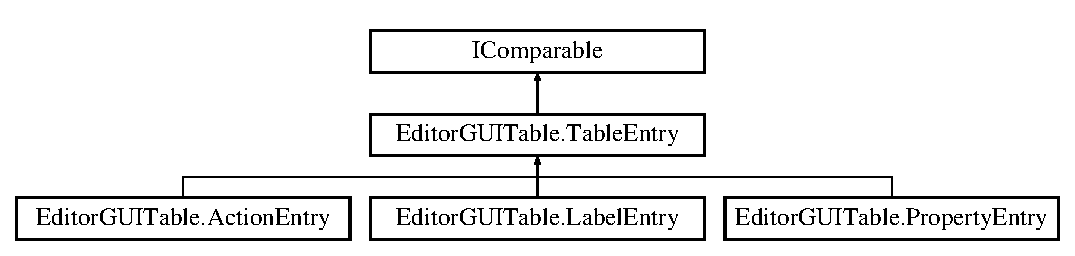
\includegraphics[height=2.994653cm]{class_editor_g_u_i_table_1_1_table_entry}
\end{center}
\end{figure}
\subsection*{Public Member Functions}
\begin{DoxyCompactItemize}
\item 
abstract void \mbox{\hyperlink{class_editor_g_u_i_table_1_1_table_entry_abe1e2747e56d50731eeec28635b366a1}{Draw\+Entry\+Layout}} (float width, float height)
\begin{DoxyCompactList}\small\item\em Draws the entry using G\+U\+I\+Layout. \end{DoxyCompactList}\item 
abstract void \mbox{\hyperlink{class_editor_g_u_i_table_1_1_table_entry_ae02e641122da6dd161d61a20576812ca}{Draw\+Entry}} (Rect rect)
\begin{DoxyCompactList}\small\item\em Draws the entry using G\+UI (without G\+U\+I\+Layout). \end{DoxyCompactList}\item 
\mbox{\Hypertarget{class_editor_g_u_i_table_1_1_table_entry_a6545f137420db34b649873ff8d7b7b51}\label{class_editor_g_u_i_table_1_1_table_entry_a6545f137420db34b649873ff8d7b7b51}} 
virtual int {\bfseries Compare\+To} (object other)
\end{DoxyCompactItemize}
\subsection*{Properties}
\begin{DoxyCompactItemize}
\item 
\mbox{\Hypertarget{class_editor_g_u_i_table_1_1_table_entry_a512ab46a9b994edfcf3a9d43a7496516}\label{class_editor_g_u_i_table_1_1_table_entry_a512ab46a9b994edfcf3a9d43a7496516}} 
abstract string {\bfseries comparing\+Value}\hspace{0.3cm}{\ttfamily  \mbox{[}get\mbox{]}}
\end{DoxyCompactItemize}


\subsection{Detailed Description}
Base class for all table entries. Draw\+Entry needs to be overriden to draw the entry for the cell. Use this to customize the table however needed. Compare\+To can be overriden to customize the sorting. comparing\+Value is used as a fallback for sorting any types of entries, even different types. 



\subsection{Member Function Documentation}
\mbox{\Hypertarget{class_editor_g_u_i_table_1_1_table_entry_ae02e641122da6dd161d61a20576812ca}\label{class_editor_g_u_i_table_1_1_table_entry_ae02e641122da6dd161d61a20576812ca}} 
\index{Editor\+G\+U\+I\+Table\+::\+Table\+Entry@{Editor\+G\+U\+I\+Table\+::\+Table\+Entry}!Draw\+Entry@{Draw\+Entry}}
\index{Draw\+Entry@{Draw\+Entry}!Editor\+G\+U\+I\+Table\+::\+Table\+Entry@{Editor\+G\+U\+I\+Table\+::\+Table\+Entry}}
\subsubsection{\texorpdfstring{Draw\+Entry()}{DrawEntry()}}
{\footnotesize\ttfamily abstract void Editor\+G\+U\+I\+Table.\+Table\+Entry.\+Draw\+Entry (\begin{DoxyParamCaption}\item[{Rect}]{rect }\end{DoxyParamCaption})\hspace{0.3cm}{\ttfamily [pure virtual]}}



Draws the entry using G\+UI (without G\+U\+I\+Layout). 


\begin{DoxyParams}{Parameters}
{\em rect} & Rect.\\
\hline
\end{DoxyParams}


Implemented in \mbox{\hyperlink{class_editor_g_u_i_table_1_1_property_entry_a176094e41cb53be100106c1d58763607}{Editor\+G\+U\+I\+Table.\+Property\+Entry}}, \mbox{\hyperlink{class_editor_g_u_i_table_1_1_action_entry_a84dfbc114f27c8108899c3c25803ae60}{Editor\+G\+U\+I\+Table.\+Action\+Entry}}, and \mbox{\hyperlink{class_editor_g_u_i_table_1_1_label_entry_a94247717318efb4e51347519e0b985dc}{Editor\+G\+U\+I\+Table.\+Label\+Entry}}.

\mbox{\Hypertarget{class_editor_g_u_i_table_1_1_table_entry_abe1e2747e56d50731eeec28635b366a1}\label{class_editor_g_u_i_table_1_1_table_entry_abe1e2747e56d50731eeec28635b366a1}} 
\index{Editor\+G\+U\+I\+Table\+::\+Table\+Entry@{Editor\+G\+U\+I\+Table\+::\+Table\+Entry}!Draw\+Entry\+Layout@{Draw\+Entry\+Layout}}
\index{Draw\+Entry\+Layout@{Draw\+Entry\+Layout}!Editor\+G\+U\+I\+Table\+::\+Table\+Entry@{Editor\+G\+U\+I\+Table\+::\+Table\+Entry}}
\subsubsection{\texorpdfstring{Draw\+Entry\+Layout()}{DrawEntryLayout()}}
{\footnotesize\ttfamily abstract void Editor\+G\+U\+I\+Table.\+Table\+Entry.\+Draw\+Entry\+Layout (\begin{DoxyParamCaption}\item[{float}]{width,  }\item[{float}]{height }\end{DoxyParamCaption})\hspace{0.3cm}{\ttfamily [pure virtual]}}



Draws the entry using G\+U\+I\+Layout. 


\begin{DoxyParams}{Parameters}
{\em width} & Width.\\
\hline
{\em height} & Height.\\
\hline
\end{DoxyParams}


Implemented in \mbox{\hyperlink{class_editor_g_u_i_table_1_1_property_entry_a5930e1e0e8cf4954cdbf25ef72e815f8}{Editor\+G\+U\+I\+Table.\+Property\+Entry}}, \mbox{\hyperlink{class_editor_g_u_i_table_1_1_label_entry_a1bf901bb1f193f4c7ff842d898968572}{Editor\+G\+U\+I\+Table.\+Label\+Entry}}, and \mbox{\hyperlink{class_editor_g_u_i_table_1_1_action_entry_ae556137b72e1e356a2e4cf4a12b88336}{Editor\+G\+U\+I\+Table.\+Action\+Entry}}.



The documentation for this class was generated from the following file\+:\begin{DoxyCompactItemize}
\item 
Editor/\+Entries/Table\+Entry.\+cs\end{DoxyCompactItemize}

%--- End generated contents ---

% Index
\backmatter
\newpage
\phantomsection
\clearemptydoublepage
\addcontentsline{toc}{chapter}{Index}
\printindex

\end{document}
